% !TeX spellcheck = hu_HU
% !TeX encoding = UTF-8

% TODO: struktúra meghatározása
\chapter{Saját munka bemutatása}
\label{chap:testenv}

\section{Kialakítani kívánt környezet meghatározása}
Dolgozatomban egy kisebb léptékű, de a fontosabb elvek ismertetését kellő mértékben lehetővé tevő tesztkörnyezetet fogok kialakítani és részletesen bemutatni. A tesztkörnyezetben egy fizikai gépen (virtual host, dom0) fogok virtuális gépeket kialakítani a \acrshort{kvm} hypervisor segítségével. Ezen környezet célja, hogy betekintést engedjen a nagyvállalati környezetek kialakításának fontosabb lépéseibe. Ahogy arról a bevezetés során szó volt, ilyen környezetekben nem ritka, hogy több száz vagy több ezer gépet kell kezelnünk. Nyilvánvaló, hogy ilyen nagyságrendű rendszert nem lehet kizárólag manuális megoldásokkal kezelni, nem várhatjuk el a rendszergazdáktól és az üzemeltetést végző mérnököktől, hogy egy-egy frissítést minden gépen külön-külön telepítsenek: ehhez sok esetben nem is adottak a lehetőségek, hiszen a legtöbb ilyen számítógép egy adatközpontban fut, ahova a biztonsági előírások miatt nem tudna minden munkatárs bejutni, továbbá körülményes lenne az egyes számítógépekhez külön-külön perifériákat csatlakoztatni, amire például a nagyobb operációsrendszer-verzióváltások során szükség lehetne az úgynevezett \textit{offline upgrade}-ek miatt -- ilyen helyzetekben a távoli elérés (pl. \acrshort{ssh}, \acrshort{vnc}) sem jelent megoldást.

Mindezen okok miatt a dolgozatomban egy infrastruktúramenedzsment eszközt fogok használni, amivel növelhető az egyes kiszolgálók karbantartásának hatékonysága mind fizikai, mind pedig virtuális gépek esetén.

\section{Fizikai gép ismertetése}

\section{Operációs rendszer}
Értekezésemben nagy szerepe lesz a választott operációs rendszereknek, hiszen ezek fognak a virtualizációs rendszer alapjául szolgálni, valamint képesnek kell lennünk a gépek távoli menedzsmentjére is, így mindenképpen olyan megoldásra van szükség, amely jól támogatott a választott infrastruktúramenedzsment eszköz által. Fontos szempont volt továbbá, hogy a tesztkörnyezet a lehetőségekhez mérten jól reprezentálja a nagyvállalati környezetben használatos rendszereket, így sok olyan OS-verzió kikerült a lehetőségek közül, amelyek ugyan népszerűek például asztali megoldásként, de egyes nagyvállalati szoftverek (legyen az adatbázismotor, vagy bizonyos eszközvezérlők, driverek) hivatalosan nem támogatottak rajtuk. Emiatt az operációs rendszerek kiválasztása során körültekintően jártam el, több Linux-disztribúció is szóba került, az ezekről született konklúziót itt foglalom össze néhány mondatban.

\subsection{\acrshort{os}-kiválasztás folyamata}
Ahogy \aref{sect:os}. alfejezetben is kitértem rá, a nagyvállalatok elsősorban a Red Hat és a SUSE Linux-disztribúciók közül választanak, hiszen ezeknek a velük együtt járó támogatás és a szoftvercsomagok széleskörű támogatottsága miatt kényelmesebb és hatékonyabb az üzemeltetésük, valamint biztonsági szempontból is kedvezőbbek (például gyorsabban kapnak meg bizonyos frissítéseket, patcheket). Szintén jobban támogatottak ezeken a rendszereken a különböző felhasználásspecifikus modulok, például \acrfull{ha}, live patching (támogatás pl. kritikus kernel biztonsági javítások telepítése a számítógép újraindítása nélkül) és real time computing (valós idejű, nagy időbeli pontosságot igénylő alkalmazások futtatására alkalmas környezet).

A fent ismertetett szélesebb körű támogatottság miatt a tesztkörnyezethez használni kívánt operációs rendszerek köre a Red Hat-re és a SUSE Linuxra korlátozódott. A végső döntésben végül az alábbi szempontok segítettek:
\begin{itemize}
	\item a tesztkörnyezetet szerettem volna egy ökoszisztémán belül tudni mind a virtuális gépeket futtató, mind pedig az azokon futó \acrshort{os}-ek esetében,
	\item könnyebb konfigurálhatóság: mivel több gépet kellett telepíteni, így fontos szerepe volt annak, hogy egy-egy operációs rendszer telepítése milyen bonyolultságú,
	\item a környezetet a költségek minimalizálása mellett szerettem volna létrehozni, így lényeges szempont volt, hogy az adott rendszerhez ne kelljen előfizetést vásárolni, mégis a lehető legközelebb álljon a kereskedelmi forgalomban kapható termékekhez
\end{itemize}

Mindezek figyelembevételével és korábbi tapasztalataim alapján a SUSE termékcsaládja mellett döntöttem. A támogatással rendelkező, előfizetéses modellt használó nagyvállalati változat mellett szabadon beszerezhető openSUSE operációsrendszer-család megfelelt a tesztkörnyezettel szemben támasztott elvárásaimnak. A rendszer telepítését és a későbbi konfigurációt a YaST keretrendszer segíti, mely számos moduljával (pl. particionálás, hálózati és tűzfalbeállítások) nagyban hozzájárul a gépek könnyebb beállításához, kezeléséhez. A YaST -- mivel szervereken való használatra tervezték, melyek gyakran nem rendelkeznek grafikus felülettel -- \aref{fig:yast-partitioner} ábrán látható megjelenés mellet egy konzolos, GUI-szerű (GUI-like) felülettel is rendelkezik, így a konfiguráció kényelmesen elvégezhető konzolos hozzáférés, például \acrshort{ssh} használata esetén is.

% TODO: yast kép olvashatóság ellenőrzése
\begin{figure}[!ht]
	\centering
	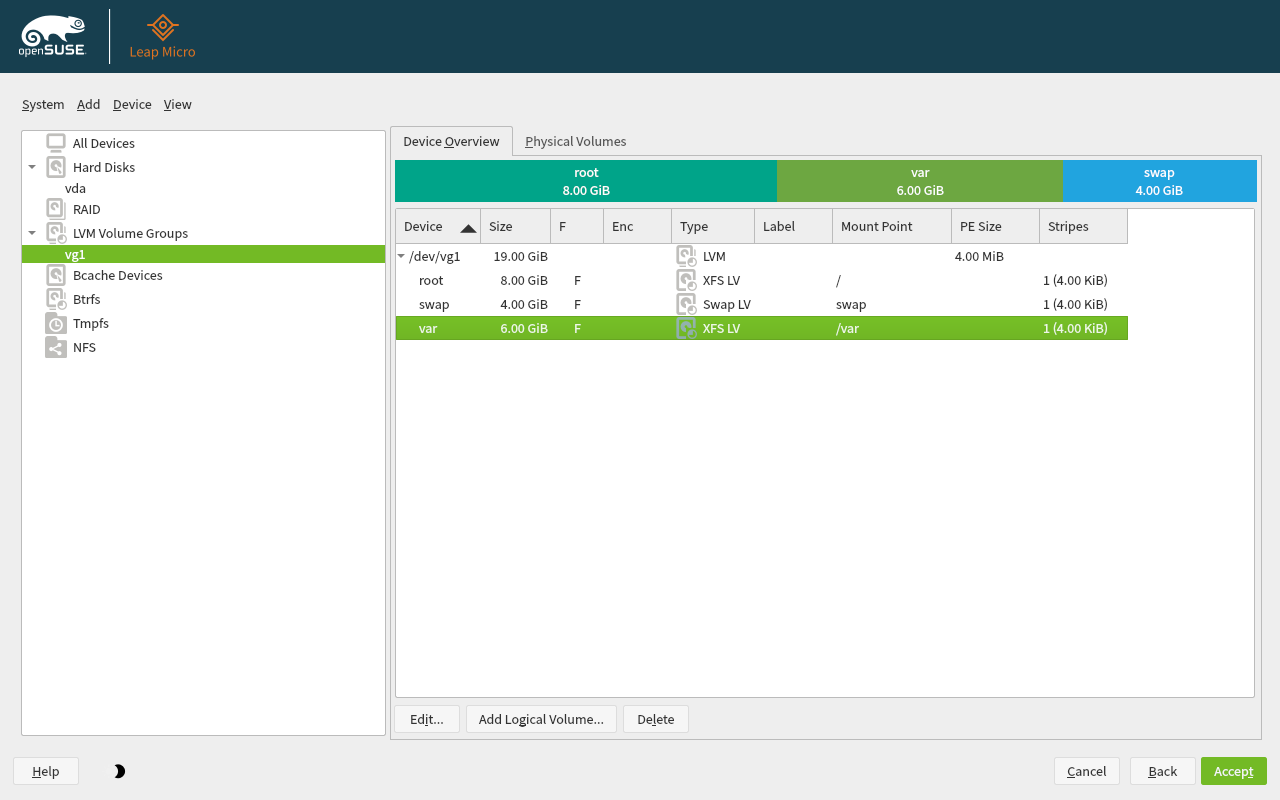
\includegraphics[width=15cm]{figures/yast-partitioner.png}
	\caption{\acrshort{lvm}-kötetek létrehozása openSUSE Leap Micro telepítése során grafikus YaST telepítő segítségével.}
	\label{fig:yast-partitioner}
\end{figure}

Az openSUSE-projekt több operációs rendszert is fejleszt\footnote{\url{https://get.opensuse.org/}}, ezek közül én a tesztkörnyezetben kettőt használtam, melyeket a következő alfejezetekben ismertetek.

\subsubsection{openSUSE Leap}
A Leap egy hagyományos értelemben vett szerver operációs rendszer. Gyakran kap biztonsági frissítéseket, új verziói pedig körülbelül évente jelennek meg. Alapjául a \acrlong{sle} szolgál, melynek előnye, hogy a két rendszer csomagjai binárisan kompatibilisek egymással, azaz egy \acrshort{sle}-rendszerre készített csomag garantáltan használható openSUSE Leap-en is, és fordítva~\cite{openSUSELeap15SP3intro}~\cite{SLE15SP3intro}. Utóbbi előnye, hogy így számos, a közösség (akár a hivatalos openSUSE projekt, akár a felhasználók) által készített csomagot használhatunk a \acrshort{sle}-alapú rendszerünkön is, bár ehhez nem kapunk hivatalos támogatást.

A nagyvállalati rendszerből való leszármazás másik nagy előnye, ami fontos volt számomra a kiválasztási folyamat során, hogy így gyakorlatilag a \acrlong{sle} egy ingyenes verzióját használhatom, mely lényegében teljesen megegyezik a vállalati környezetben használt megoldással, és előfizetés nélkül is kap frissítéseket, így folyamatosan naprakészen tartható. A biztonsági javításokat illetően fontos megjegyezni, hogy a Leap rendelkezik egy olyan csomagforrással (repository) is, mely a \acrlong{sle}-ban is elérhető frissítéseket tartalmazza, így az ott hozzáférhető fontos javításokat is telepíthetjük a Leap-et futtató rendszereinkre~\cite{openSUSELeapSLERepo}.

\subsubsection{openSUSE MicroOS}

\section{Gépmenedzsment: Salt}


\section{Monitoring}

\section{Továbbfejlesztési lehetőségek}